%! Author = adnansiddiquei
%! Date = 05/03/2024

% Preamble
\documentclass[a4paper,11pt]{article}
\pdfoutput=1

% Packages
%\usepackage[colorlinks=true, linkcolor=blue, urlcolor=blue, citecolor=blue, pdfborder={0 0 0}]{hyperref}
\usepackage{url}
\usepackage{jcappub}
\usepackage[T1]{fontenc}
\usepackage{listings}
\usepackage{roboto}
\usepackage{subcaption}
\usepackage{blindtext}
\usepackage{seqsplit}
\usepackage[nottoc]{tocbibind}

%\newcommand{\inlinecode}[1]{\lstinline{#1}}
%\newcommand{\inlinecode}[1]{\texttt{#1}}
\newcommand{\inlinecode}[1]{\texttt{\seqsplit{#1}}}
\lstset{basicstyle=\fontfamily{pcr}\selectfont}


\title{\boldmath Reproducing AstroCLIP: An Evaluation on Cross-Modal Pre-Training for Astronomical Foundation Models}

% %simple case: 2 authors, same institution
\author{Adnan Siddiquei}
\affiliation{University of Cambridge}

% e-mail addresses: one for each author, in the same order as the authors
\emailAdd{as3438@cam.ac.uk}
\note{Word Count: XXXXX (including figure captions and appendix).}


\begin{document}
    \maketitle
    \flushbottom


    %! Author = adnansiddiquei
%! Date = 04/06/2024

\section{Introduction}

    %! Author = adnansiddiquei
%! Date = 04/06/2024

\section{Original AstroCLIP Paper}\label{sec:original-paper}
The original AstroCLIP paper~\cite{astroclip} whose results we reproduce in this paper, implemented a multi-modal contrastive
learning approach to embed galaxy spectra and galaxy images into a shared latent space.
This implementation utilised a transformer-based spectrum embedder and a convolutional image embedder to project the two
modalities into a shared 128-dimensional embedding, and further showed that the learned embeddings were well-aligned
with the physical properties of the galaxies.
The authors demonstrated that the learned embeddings could be used to make relatively accurate zero-shot predictions on
redshift and stellar mass of galaxies using k-NN regression.
For ease of comparison, we provide a brief overview of the implementation details and key results of the original
AstroCLIP paper.

\paragraph{Data} The galaxy image data used by the authors~\citep{astroclip} was curated from the DESI Legacy Survey Data
Release 9~\citep{desilegacy2018}, as prepared by~\cite{stein2021}.
This was cross-referenced to the DESI Early Data Release~\citep{desiearly2023} to obtain the corresponding galaxy spectra,
and cross-referenced to the PRObabilistic Value-Added Bright Galaxy Survey (PROVABGS) Catalog~\citep{provabgs2021}
to obtain the redshift and stellar mass labels for the galaxies - yielding a total of 197,976 galaxy spectra and image pairs.

\paragraph{Spectrum Embedder} The authors pre-trained a transformer-based spectrum embedder using a self-supervised mask
filling task on the galaxy spectra.
All the weights of this embedder were then frozen and a single cross-attention layer followed by an MLP was added to project
the spectrum into a 128-dimensional embedding, yielding a total of 362k trainable parameters.

\paragraph{Image Embedder} The pre-trained convolutional image embedder was acquired from~\cite{stein2021}.
This image embedder had a ResNet-50 architecture and was trained with a self-supervised method on a sample of 3.5 million
galaxy images (augmented in a variety of ways) from the DESI Legacy Survey~\citep{desilegacy2018} using the MoCo v2
framework~\citep{moco2020, mocov22020} in order to embed the images into a 128-dimensional space.
This image embedder had the convolutional layers frozen and yielding a total of 4.5M trainable parameters in the final
dense layers of the model.

\paragraph{Training} The authors used a contrastive learning approach to learn a shared embedding space for the images
and spectra.
A variety of augmentations were applied to the images and spectra and the respective embedders were trained using an
InfoNCE loss~\citep{infonce2020} over 15,000 iterations with a batch size of 512.

\paragraph{Key Results} The authors demonstrated that the embeddings were well-aligned in 2 main ways:
In-modal and cross-modal similarity searches using cosine similarity showed that two 'cosine similar' galaxies yielded
similar spectra and images.
Secondly, zero-shot regression of redshift and stellar mass using k-NN regression on the learned embeddings similarly
yielded relatively accurate predictions.
These are both further discussed in XXXXX when we compare the results of our reproduction with the original paper.

    %! Author = adnansiddiquei
%! Date = 04/06/2024

\section{Related Works}\label{sec:related-works}

    %! Author = adnansiddiquei
%! Date = 04/06/2024

\section{Method}\label{sec:method}
\subsection{Objective}\label{subsec:objective}
As per the original AstroCLIP implementation~\citep{astroclip}, the objective of this piece of work was to embed galaxy
spectra and galaxy images into a shared latent space using a multi-modal contrastive learning approach.
This follows on naturally from the assumption that the two modalities are different physical representations of the same
underlying object, and as such should be able to be represented in a shared, lower dimensional space.
The aim of this reproduction was to

\subsection{Implementation}\label{subsec:implementation}
Our implementation did not differ too greatly from the original AstroCLIP implementation~\citep{astroclip}.
We created our AstroCLIP model with a pretrained image and spectrum embedder, and then fine-tune the model using contrastive
learning under the InfoNCE loss to learn a shared 128-dimensional embedding space for the two modalities.
To acquire the pretrained embedders, the fine-tuned embedders or the dataset used, we refer the reader to the referenced
literature or to our codebase which contains all the necessary details.

\paragraph{Spectrum Embedder} We acquired a pre-trained spectrum embedder from the works of~\cite{liang2023} who used
a convolutional autoencoder to learn a 6-dimensional embedding for galaxy spectra using the Bright Galaxy Survey of the
DESI Early Data Release~\citep{desiearly2023}, for precise details on architecture and training, see the original paper.
The encoder consisted of a series of convolutional layers followed by 4 fully-connected layers.
The last 3 of these layers were deleted and replaced with a single fully-connected layer to project the output of the first
layer into a 128-dimensional embedding\footnote{That is to say, in the edited model, the first fully-connected layer took
256 inputs and output 128-dims into the second layer which also output 128-dims.
The first layer contained pre-trained weights, the second layer was randomly initialised.}.
The entire model contained 3.2M parameters, all of which were set as trainable parameters, differing to the implementation
by~\cite{astroclip} where the authors set only the final fully-connected layers of their pre-trained transformer-based spectral
embedder as trainable.
The spectra were normalised in the same way as done by~\cite{liang2023}\footnote{The spectra were normalised over their median
flux in the rest-frame wavelength range of $[5300, 5850]$, where the rest-frame spectra were computed by assuming all
spectra were redshifted by exactly $z=0.8$.} and then noise was added to the spectra using a
similar technique as utilised by~\cite{astroclip}\footnote{Noise added to the spectra at any point was Gaussian and scaled
by the distribution of values at any given flux measurement.
Measurements at wavelengths with more variance therefore had more noise added.}.

\paragraph{Image Embedder} The image embedder we used was the same as the one used by~\cite{astroclip}, courtesy of
\cite{stein2021}, see Section~\eqref{sec:original-paper} for further details.
However, unlike~\cite{astroclip} who only fine-tuned the fully-connected layers, we once again chose to set all 28.0M parameters
of the model as trainable.
The images were transformed and augmented using the same techniques used in the original AstroCLIP paper; the 3-channel (g, r, z)
152x152 pixel images were augmented with Gaussian noise, rolled, rotated and flipped randomly before being cropped to the central
96x96 pixels.
This was then converted from (g, r, z) to RGB using the same scaling method utilised by~\cite{stein2021}.
The conversion to RBG was relatively arbitrary and did not change meaning of the image, but was done to ensure the images
were in the same format as expected by the pre-trained image embedder.

\paragraph{Data} We use the same dataset as curated and helpfully provided by \cite{astroclip}, see Section~\eqref{sec:original-paper}
for further details.
This consists of 197,976 galaxy spectra and image pairs, along with their redshift measurements.
The data was then further pre-processed to drop any galaxies with spectra outside the range $[0, 0.8]$ which was in line with the
pre-training of the spectrum embedder, but is a larger range than utilised by \cite{astroclip} who used $[0, 0.6]$ in their final results.
Additionally, some of the galaxy spectra in the dataset were completely flat (exactly 0 flux across all wavelengths)
and so these galaxies were dropped from the dataset.
This resulted in a total of 3,241 (1.6\%) image-spectra pairs being removed in the pre-processing step.
The dataset was then split into a training and validation set, with 80\% of the data used for training and 20\% for
validation; all results displayed in this paper were performed on the validation set.

    %! Author = adnansiddiquei
%! Date = 04/06/2024

\section{Results}\label{sec:results}
To assess and demonstrate the performance of our AstroCLIP model, we reproduce a subset of the downstream tasks from
the original implementation.
The held-out validation set (composing of 39,599 of the 197,976 image-spectra pairs) was used to evaluate the performance
by assessing the accuracy of zero-shot k-NN redshift estimations and qualitative similarity retrieval tasks.
Notation used in this section intentionally follows that of the original paper for the reader's convenience.

\subsection{Zero-shot k-NN Redshift Estimation}\label{subsec:results-redshift-regression}
\begin{figure}[htb]
    \centering
    \makebox[\textwidth]{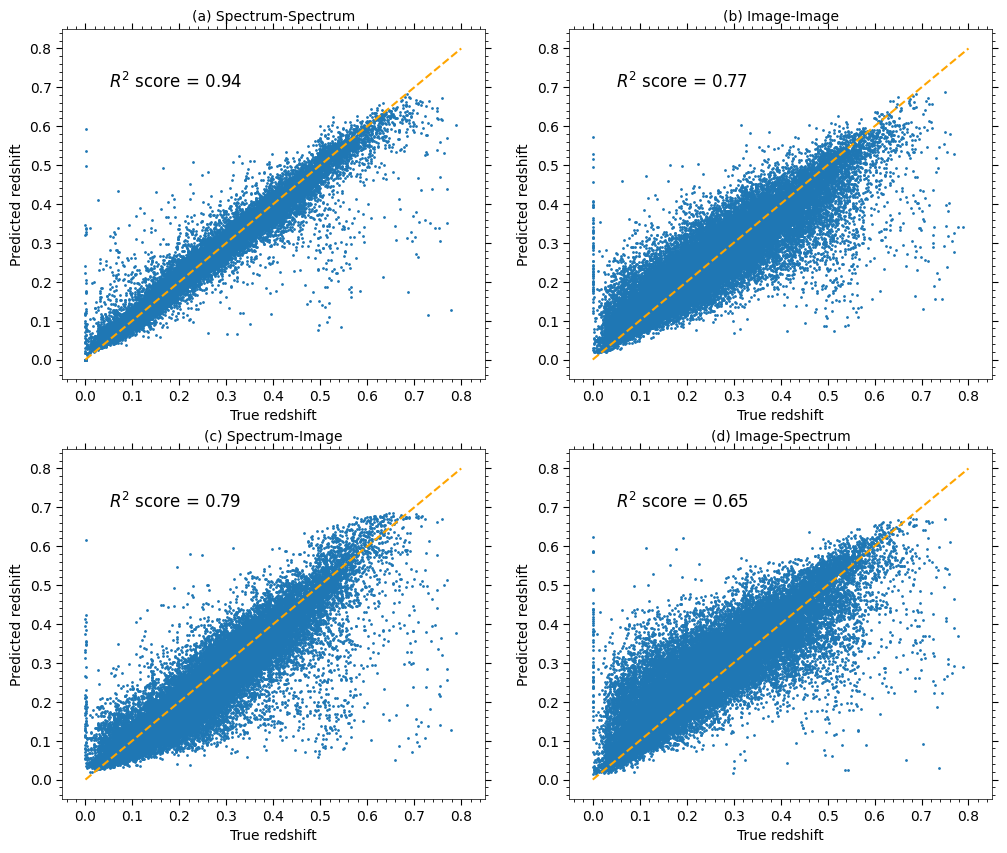
\includegraphics[width=1.2\textwidth]{figures/redshift_knn_regression}}
    \caption{In-modal and cross-modal zero-shot redshift predictions using k-NN regression on the learned embeddings. The y-axis shows
    the predicted redshift (the average of the 16 closest neighbours in terms of Euclidean distance) and the x-axis shows the true redshift.
    The dashed line represents a perfect prediction, and the $R^{2}$ of the fit is shown in the top left corner.
    $S_{kNN}(\mathbf{z}_{q}^{sp}, \mathbf{z}^{im})$ indicates the cross-modal prediction where a spectrums redshift was
    predicted using its 16 closes image embedded neighbours.}
    \label{fig:rkr}
\end{figure}

Figure~\eqref{fig:rkr} shows the zero-shot redshift predictions using k-NN regression on the learned embeddings for
both in-modal (spectrum to spectrum, image to image) and both cross-modal (spectrum to image, image to spectrum) predictions.
Both the spectrum-spectrum and image-image in-modal predictions fall slightly short of the predictive power of the
model trained by~\cite{astroclip} with our model achieving $R^{2}$ values of 0.94 and 0.74 respectively, compared to
0.79 and 0.98.
This is yields in interesting comparison on the effectiveness of the underlying architectures used, as well as pre-training
strategy.
The image and spectrum embedders utilised here were both CNNs and pre-trained as described in XXXXXXX, compared
to the transformer structure used in the original paper.
State-of-the-art galaxy spectra models thus far have traditionally been modelled using 1D convolutional architectures,
such as the one we have implemented in our AstroCLIP implementation.
A similar statement can be made on image embedders which have been traditionally modelled using 2D convolutional architectures.
However, these results indicate that the transformer architecture may be more effective in learning the underlying
representations of the data, as the original paper's model outperforms our implementation in both in-modal predictions.
Likewise, the pre-training performed by~\cite{astroclip} may have also been a more effective strategy for transfer learning
on this task XXXX WHAT IS THE PRE-TRAINING? WHAT METHODS WERE USED? XXXX.

\subsection{Retrieval by Cosine Similarity}\label{subsec:results-retrieval}
\begin{figure}[htb]
    \centering
    \makebox[\textwidth]{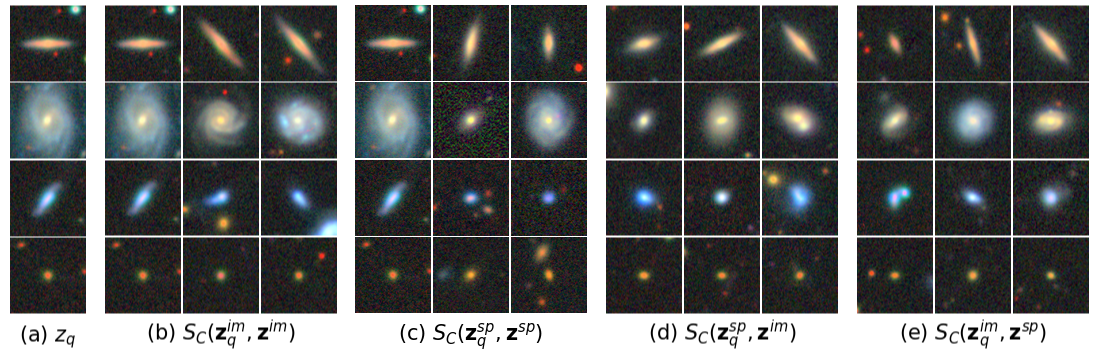
\includegraphics[width=1.2\textwidth]{figures/sim_search_images_all}}
    \caption{In-modal and cross-modal similarity search using cosine similarity on the learned embeddings.
        (a) shows the query galaxies; (b) shows the 3 most similar galaxies using an in-modal image to image search; and
        so on.
        By construction, the most similar in-modal galaxy to any given galaxy is itself, hence, the first column of images
        in (b) and (c) are identical to the query image in (a).}
    \label{fig:ssia}
\end{figure}

\begin{figure}[htb]
    \centering
    \makebox[\textwidth]{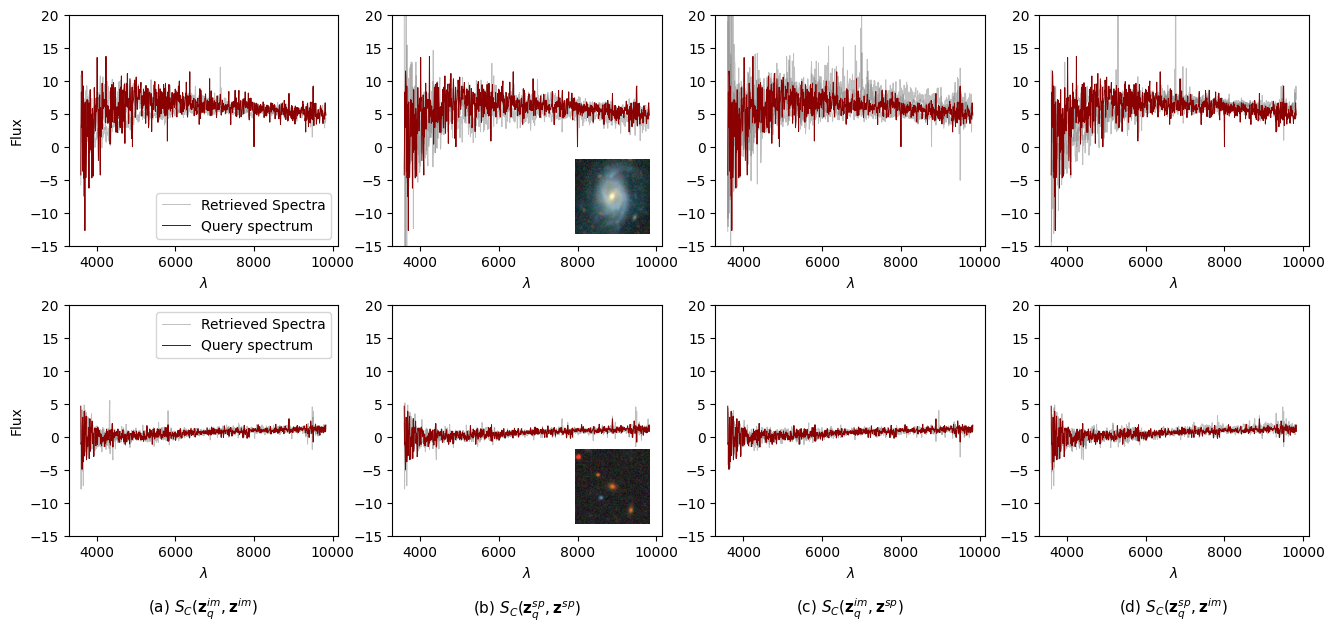
\includegraphics[width=1.2\textwidth]{figures/sim_search_spectra}}
    \caption{Similar to Figure~\eqref{fig:ssia}, each row in this figure depicts a single query galaxy (query spectrum in red,
        galaxy imaged in plot (b)), with each subfigure showing the spectrum of the 3 most cosine similar galaxies to the
        query galaxy by in-modal and cross-modal similarity search.}
    \label{fig:sss}
\end{figure}


    \clearpage

%    \nocite{*}
    \bibliographystyle{apalike}
    \bibliography{main}
    \clearpage

    %\appendix

    %\section{Appendix A}\label{app:app-a}
    %Lorem ipsum dolor sit amet, consectetur adipiscing elit. Suspendisse eget urna laoreet, elementum tellus nec, dapibus dui.
\end{document}
